% !TeX root = ../main.tex
\chapter{Metodología}
\label{cap:metodologia}

Este capítulo describe cómo se ha llevado a cabo el trabajo. Un proyecto como VH SimGrid combina dos naturalezas distintas. Por un lado, tiene un componente de investigación, porque se quiere comprobar si un ecosistema de simracing de fabricación propia puede ofrecer prestaciones comparables a las de los equipos comerciales de gama media. 
Por por otro, es un desarrollo de ingeniería de cierta envergadura, con tres periféricos, sus firmwares y una aplicación de escritorio que deben avanzar de forma coordinada. Por ello se distinguen dos niveles metodológicos. 
La metodología de investigación (sección~\ref{sec:metodologia-investigacion}) fija las etapas por las que pasa el trabajo, desde la identificación del problema hasta la comunicación de los resultados. La metodología de gestión (sección~\ref{sec:metodologia-gestion}) organiza el día a día del desarrollo dentro de esas etapas. Por último, se presentan las herramientas empleadas para aplicar dicha gestión (sección~\ref{sec:herramientas}).

%======================================================================
\section{Design Science Research}
\label{sec:metodologia-investigacion}

El trabajo sigue la metodología \emph{Design Science Research} (DSR), propia de la ingeniería y de los sistemas de información \parencite{hevner_2004_dsr,peffers_2007_dsrm}. La DSR busca resolver un problema real mediante la creación de un \emph{artefacto}, es decir, un producto, sistema o método nuevo que se diseña, se construye y se evalúa con rigor. El conocimiento surge de ese proceso de diseño y de la evaluación del resultado.

Este enfoque encaja con el proyecto. El problema de partida es práctico: los periféricos de simracing de gama media son caros, cerrados y carecen de un software común (capítulo~\ref{cap:problema-solucion}). La respuesta es un artefacto concreto, el ecosistema VH SimGrid, cuya validez solo puede juzgarse construyéndolo y probándolo sobre hardware real con simuladores comerciales.

\Textcite{hevner_2004_dsr} describen la DSR mediante tres ciclos que se aplican de forma natural a este trabajo:

\begin{itemize}
	\item \textbf{Ciclo de relevancia}: conecta el artefacto con el entorno en el que se usará. Aquí, las necesidades del piloto aficionado y los requisitos que imponen los simuladores, Windows y el estándar USB HID \parencite{usb_hid_pid}.
	\item \textbf{Ciclo de rigor}: apoya el diseño en el conocimiento existente. En este caso, el estado del arte de los periféricos comerciales y de fabricación propia, el control de motores sin escobillas mediante FOC y los proyectos abiertos de referencia, como ODrive \parencite{odrive_github} y OpenFFBoard \parencite{openffboard_github}.
	\item \textbf{Ciclo de diseño}: alterna la construcción y la evaluación del artefacto hasta que cumple los objetivos fijados.
\end{itemize}

Para ordenar el proceso se ha adoptado el modelo de seis etapas propuesto por \textcite{peffers_2007_dsrm}, que se aplica al proyecto como se describe a continuación:

\begin{enumerate}
	\item \textbf{Identificación del problema y motivación.} Se analiza la situación del simracing doméstico: el coste de los equipos de gama media, la dependencia de software propietario y la dispersión de las herramientas de apoyo al piloto en programas separados. Esta etapa se apoya en el estudio del estado del arte (capítulo~\ref{cap:estado-arte}) y da lugar al planteamiento del problema (capítulo~\ref{cap:problema-solucion}).
	
	\item \textbf{Definición de los objetivos de la solución.} A partir del problema se establece qué debe conseguir el artefacto. Se fijan los tres objetivos generales del trabajo, desarrollar los periféricos, desarrollar la aplicación y validar el ecosistema, y se desglosan en objetivos específicos medibles (capítulo~\ref{cap:objetivos}).
	
	\item \textbf{Diseño y desarrollo.} Se diseña la arquitectura del ecosistema y se construyen sus partes: la electrónica y la mecánica de cada periférico, sus firmwares y la aplicación de escritorio con sus módulos de configuración, dash, ingeniero de pista y análisis de telemetría. Es la etapa más extensa y la que concentra la mayor parte del esfuerzo.
	
	\item \textbf{Demostración.} Se emplea el artefacto en el contexto para el que se ha creado: sesiones de conducción reales con los simuladores compatibles, en las que los tres periféricos y la aplicación funcionan de forma conjunta.
	
	\item \textbf{Evaluación.} Se comprueba en qué medida el artefacto cumple los objetivos de la etapa~2. Se verifica cada periférico por separado, se someten las protecciones de la base a situaciones reales, como golpes y bloqueos del volante, se valida el funcionamiento integrado y se compara el coste y las prestaciones con los equipos comerciales. Los resultados de esta etapa determinan si es necesario volver a la etapa~3.
	
	\item \textbf{Comunicación.} Se difunden el artefacto y el conocimiento obtenido. Por una parte, mediante esta memoria; por otra, mediante la publicación de las versiones del instalador y de los firmwares en el repositorio oficial del proyecto, que es su único canal de distribución.
\end{enumerate}

\begin{figure}[htbp]
	\centering
	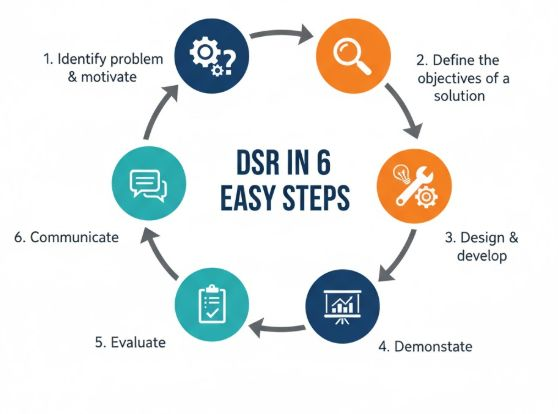
\includegraphics[width=0.75\textwidth]{img/DSR.png}
	\caption[Etapas de la metodología \emph{Design Science Research}]{Las seis etapas de la metodología \emph{Design Science Research}. Adaptado de: \parencite{peffers_2007_dsrm}}
	\label{fig:dsr-etapas}
\end{figure}

Aunque las etapas se presentan en orden, el proceso no es lineal. Las etapas 3, 4 y 5 forman un ciclo que se ha recorrido varias veces: cada prueba en pista o en el banco de trabajo ha revelado aspectos que mejorar, desde el ajuste de las protecciones del motor hasta la respuesta de los pedales o la usabilidad de la aplicación, y esas conclusiones han vuelto a la etapa de diseño. Cada vuelta completa a este ciclo se ha cerrado con una nueva versión del sistema, lo que enlaza la metodología de investigación con la de gestión que se describe a continuación.

%======================================================================
\section{Metodología Kanban}
\label{sec:metodologia-gestion}

Kanban se basa en hacer visible el trabajo. Cada tarea se representa como una tarjeta en un tablero dividido en columnas, una por cada estado por el que pasa, de modo que se ve de un vistazo qué está pendiente, qué está en marcha y qué se ha terminado. Además, se limita el número de tareas que pueden estar en curso a la vez (límite WIP, del inglés \emph{work in progress}). Una tarea nueva solo empieza cuando otra termina, lo que obliga a acabar lo empezado antes de abrir nuevos frentes. El objetivo es que las tareas avancen por el tablero de forma continua. Si se acumulan en una columna, señalan un cuello de botella que hay que resolver. A diferencia de otras metodologías ágiles, Kanban no divide el trabajo en iteraciones de duración fija ni impone roles o reuniones. Las tareas se incorporan al tablero en cuanto aparecen y se atienden por orden de prioridad, y el proceso se ajusta poco a poco según lo que muestra el propio tablero.

El tablero del proyecto tiene cuatro columnas. En \emph{Pendiente} están las tareas identificadas, ordenadas por prioridad. En \emph{En curso}, las que se están desarrollando, con un máximo de tres a la vez. En \emph{En pruebas}, las terminadas que deben validarse sobre el hardware real o en un simulador. En \emph{Hecho}, las ya validadas e integradas en el sistema. Cada tarea se etiqueta además según el subsistema al que pertenece (volante, pedalera, aro o aplicación) y según su tipo (nueva funcionalidad, corrección o documentación).

Para dar estructura al flujo continuo, las tareas se agrupan en versiones. Cada versión se cierra cuando todas sus tareas han pasado por la columna de pruebas. Se numera siguiendo el versionado semántico \parencite{semver_web} (v\emph{X}.\emph{Y}.\emph{Z}): el primer número cambia con las modificaciones incompatibles, el segundo con las funcionalidades nuevas y el tercero con las correcciones. Cada versión publicada coincide con una vuelta completa al ciclo de diseño y evaluación de la DSR.

%======================================================================
\section{Herramientas}
\label{sec:herramientas}

Para aplicar la metodología de gestión se ha utilizado \textbf{GitHub} \parencite{github_docs}, la plataforma en la que se aloja el repositorio oficial del proyecto. Reunir en un mismo sitio el tablero de tareas, el código y las publicaciones evita mantener herramientas separadas y permite enlazar directamente cada tarea con su resultado. En concreto, se han empleado las siguientes funciones:

\begin{itemize}
	\item \textbf{GitHub Projects}: proporciona el tablero Kanban con las cuatro columnas descritas en la sección~\ref{sec:metodologia-gestion}. Las tarjetas se mueven de una columna a otra a medida que avanza el trabajo, y el tablero se filtra por etiquetas para ver solo un subsistema.
	\item \textbf{GitHub Issues}: cada tarea del tablero es una incidencia (\emph{issue}) con su descripción, sus etiquetas y su historial de comentarios. Las incidencias también son el canal por el que los usuarios notifican fallos, según se indica en el apartado de soporte del repositorio, de modo que los problemas detectados por terceros entran directamente en la columna de pendientes.
	\item \textbf{Milestones}: cada versión planificada se representa como un hito al que se asignan sus incidencias. El porcentaje de incidencias cerradas indica el avance de la versión.
	\item \textbf{GitHub Releases}: cuando una versión se completa, se publica con su instalador de Windows y los firmwares de los tres periféricos. Esta función materializa la etapa de comunicación de la DSR y sirve como registro histórico de la evolución del sistema.
	\item \textbf{Git}: el control de versiones del código fuente. Cada cambio queda registrado y puede asociarse a la incidencia que resuelve, lo que permite rastrear qué modificación corresponde a cada tarea.
\end{itemize}

\begin{figure}[htbp]
	\centering
	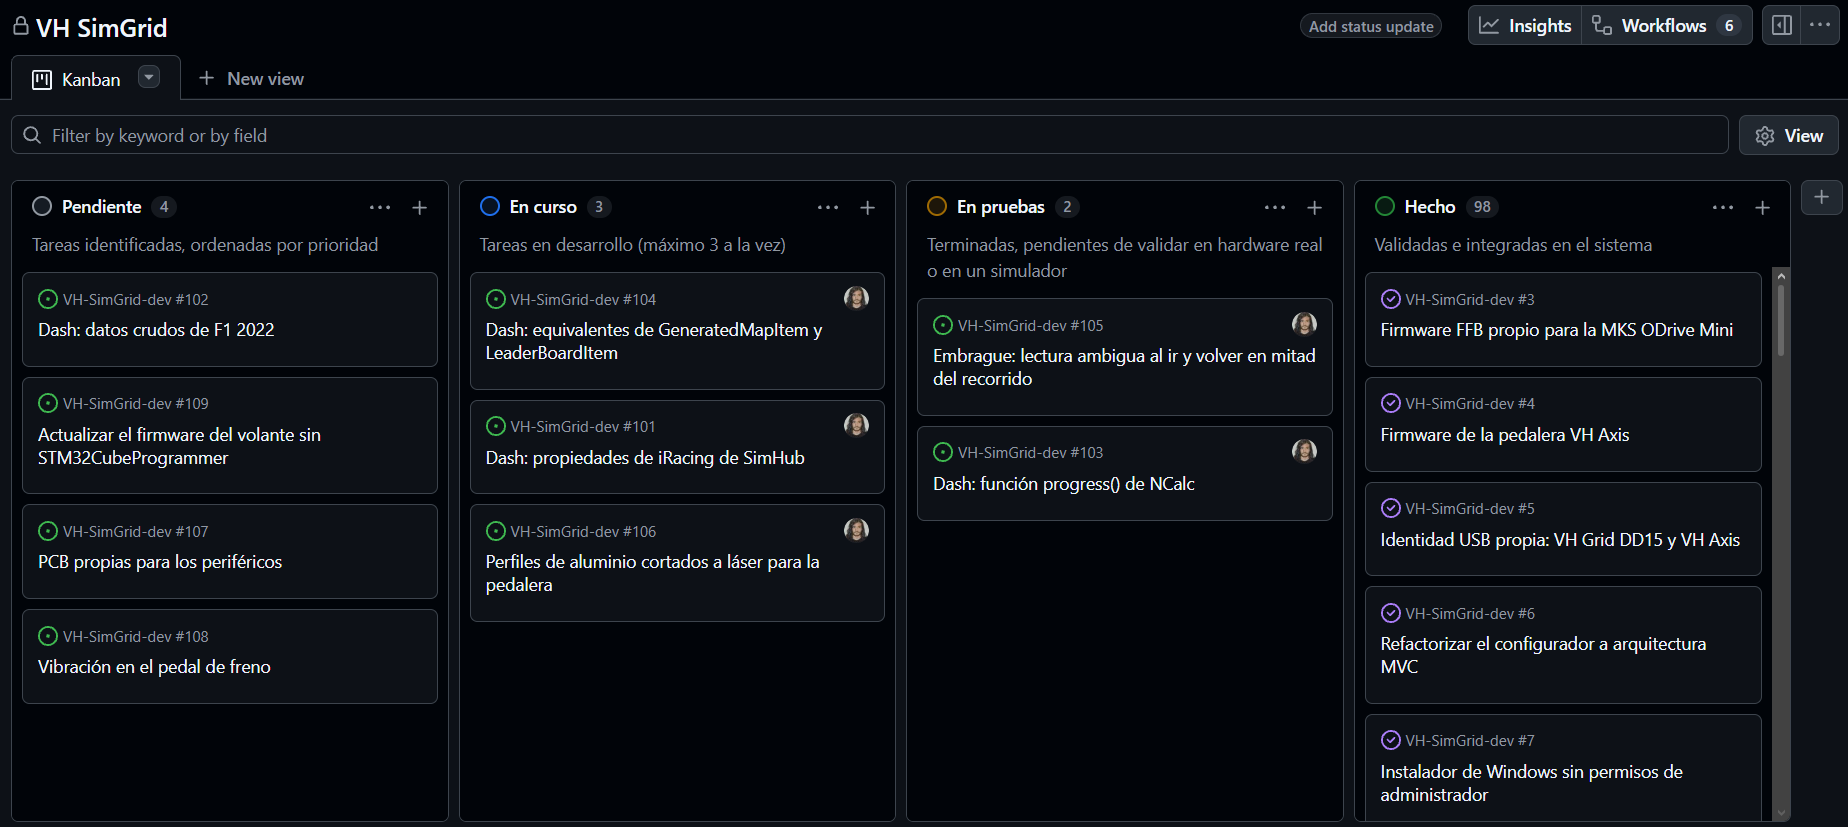
\includegraphics[width=\textwidth]{img/Kanban.png}
	\caption[Tablero Kanban del proyecto en GitHub Projects]{Tablero Kanban del proyecto en GitHub Projects, con las columnas Pendiente, En curso, En pruebas y Hecho. (Fuente propia)}
	\label{fig:kanban}
\end{figure}

En conjunto, estas herramientas cubren todo el recorrido de una tarea: su aparición como incidencia, su planificación en un hito, su seguimiento en el tablero, su implementación en el código y su entrega final en una versión publicada.